\chapter{Evaluation}
\label{chap:evaluation}

Questions the evaluation needs to answer:

\begin{enumerate}
\item Show the implementations do not impose undue performance overheads on standard microkernel
operations.
\item Show that criticality mode switch is bounded by high criticality threads.
\item Show the cost of various timeout exception recovery mechanisms.
\item Show that temporal isolation is achieved.
\item Show that deadlines can be met during and after a mode switch.
\item Show the model is practical and consistent with existing frameworks for critical software.
\end{enumerate}

\section{Hardware}

% describe benchmark setup, details of each hardware platform
We ran microbenchmarks on a variety of hardware to show the overheads of the model compared to
baseline \selfour. \Cref{t:evaluation-hardware} summarises the hardware platforms. \textsc{Sabre} is
the verified platform for \selfour, although at the time of writing verification for \textsc{x64} is
ongoing. Currently, the only platforms that support more than one core are \textsc{Sabre},
\textsc{ia32} and \textsc{x64}.

Additionally, we use several load generators running Linux on an isolated network for several
benchmarks that require a network.

\TODO{Appendix listing exact hardware details}
\begin{table}[ht]
\rowcolors{2}{gray!25}{white}
\begin{tabularx}{\textwidth}{llXlccc}\toprule
    \emph{Platform} & \emph{Arch.} & \emph{Microarchictecture} & \emph{CPU} & \emph{Clock (GHz)} &
    \emph{Mode} & \emph{Cores} \\\midrule
    \textsc{KZM}  & ARMv6          & ARM1136JF-S          & i.MX31       & 1.00         & 32  &  1 \\
    \textsc{Sabre} & ARMv7          & Cortex-A9           & i.MX6        & 1.00         & 32  & 4 \\
    \textsc{Hikey32} & ARMv8          & Cortex-A53          & Kirin 620    & 1.20         & 32  & 8 \\
    \textsc{Hikey64} & ARMv8          & Cortex-A53          & Kirin 620    & 1.20         & 64  & 8 \\
    \textsc{TX1}  & ARMv8          & Cortex-A57          & Jetson TX1   & 1.91        & 64  & 4 \\
    \textsc{atom} & x86            & E3825               & Atom         & 1.33         & 32  & 2 \\
    \textsc{ia32} & x86            & i7-4770             & Haswell      & 3.10         & 32  & 4 \\
    \textsc{x64}  & x86            & i7-4770             & Haswell      & 3.10         & 64  & 4
\\\bottomrule\hline
\end{tabularx}
\caption{Hardware platforms and specifications used in benchmarks. \textsc{Hikey32/Hikey64}
    and \textsc{ia32/x64} are the
same platform in 32 and 64 bit mode respectively.}
\label{t:evaluation-hardware}
\end{table}

\section{Overheads}

We first present a suite of microbenchmarks to evaluate any performance overheads against baseline
\selfour.
For each benchmark we ensure \gls{FPU} context switching is off by performing the required number of 
system calls 
without activating it such that the kernel will cease switching the FPU context. We present
overheads on IPC operations, signalling and interrupts, and finally scheduling. 

For each of the benchmarks in this section, we measure the cost of measurement, which is reading the
cycle counter, and subtract that from the final measurement.

\subsection{Timer}
\label{s:eval-timer}

Two of the main sources of overhead introduced by our model are related to the need to read and reprogram the timer on
non-fastpath kernel entries, and when performing a scheduling context switch. We show the results of
microbenchmarks of both of these operations in \Cref{t:evaluation-timer}, and note the timer
hardware used on the specific platform. 

\begin{table}[ht]\centering
\rowcolors{2}{gray!25}{white}
\begin{tabularx}{\textwidth}{lXccc}\toprule
    \emph{Platform} & \emph{Timer} & \emph{Read time} & \emph{Set timeout} & \emph{Sum}
    \\\midrule
    \textsc{KZM}               & General purpose timer    & 83 (0)   & 203(0)  & 286   \\
    \textsc{Sabre}             & ARM MPCore global timer  & 23 (0)   & 36 (0)  & 59    \\
    \textsc{Hikey32/64}        & ARM generic timers       &  6 (0)   &  6 (0)  & 12    \\
    \textsc{TX1}               & ARM generic timers       &  8 (0)   &  1 (0)  & 9     \\
    \textsc{atom}              & TODO                     & TODO     & TODO    & TODO  \\
    \textsc{ia32}              & TSC deadline mode        & 12 (2.2) & 220 (1.0) & 232 \\
    \textsc{x64}               & TSC deadline mode        & 11 (2.3) & 217 (2.0) & 228 \\
    \bottomrule\hline
\end{tabularx}
\caption{Latency of timer operations per platform in cycles. Standard deviations shown
in parenthesis.}
\label{t:evaluation-timer}
\end{table}

For both microbenchmarks, we read the timestamp before and after the operation, and do this 102
times, discarding the first two results to prime the cache.  We take the difference of the cycle
counts, and subtract the cost of measuring the cycle counter itself. The results show the cost of
both operations separately, and then their sum, which is the total measured overhead introduced by timers on
scheduling context switch.

All platforms excluding \textsc{KZM} have a 64-bit timer available, making \textsc{KZM} the only platform requiring
timer overflow interrupts, which are not measured as \textsc{KZM} is a deprecated platform provided for comparison
with modern ARM versions.

\textsc{Sabre} and \textsc{KZM} both use memory mapped timers, the 32-bit general purpose timer for the former and
64-bit ARM global timer for the latter. \textsc{Sabre} has four cores and the timer registers are banked,
making access fast for each core. Timer access on \textsc{Sabre} is significantly faster than the
\textsc{KZM}. 

For all other ARM platforms, the ARM generic timers are available, which are accessed via the
coprocessor. The vast majority of new ARM platforms support the generic timers. 

On \textsc{x64} we use the \gls{TSC} with \gls{TSC}-deadline
mode~\citep{Intel_64_IA-32:asdmspg_325384}, an architectural \gls{MSR} available since
Intel SandyBridge by which a local-APIC timer interrupt is triggered when the \gls{TSC} matches the
programmed value. 

While \Cref{t:evaluation-timer} shows the instruction latency of each timer operation. In practice, especially
for \textsc{x64}, these operations are subject to pipeline parallelism and out-of-order execution, which
reduces the overhead.

Results on both architectures show that the overhead of a tickless kernel, which requires the timers
to be frequently read and reprogrammed, is practical on modern hardware.

\subsection{IPC performance}

\Gls{IPC} performance is a critical measure of the practicality and efficiency of a
microkernel~\citep{Liedtke_95}. We benchmark our \gls{IPC} operations against base system, \selfour,
which has an established efficient \gls{IPC} fastpath~\citep{Elphinstone_Heiser_13}. 

To evaluate IPC performance we set up a client (the caller) and server (the callee) in different
address spaces. We take
timestamps on either side of the IPC operation being benchmarked and record the difference. This is
done 16 times for each result value to prime the cache, then record the next value. Results
presented are for performing this a total of 16 times. Additionally, we measure the overhead of
system calls stubs in the same way and subtract this from the measurement, to obtain only the kernel
cost of the operation\footnote{The \gls{IPC} benchmarks already existed for \selfour, but were modified to
    support the \gls{MCS} kernel during the work for this thesis}. The message sent is zero length, so not
neither the caller or callee's \gls{IPC} buffer accessed.
This is done for both directions of IPC, as described in \Cref{sec:seL4-api}. 

We evaluate the \gls{IPC} fastpath and two slowpath variants: slowpath between passive threads and
active threads.

\subsubsection{Fastpath}

\begin{table}[ht]\centering
\begin{tabular}{ll r@{~}l r@{~}l r@{~}r}\toprule
\emph{Platform}           & \multicolumn{1}{c}{\emph{Operation}}
                                & \multicolumn{2}{c}{\emph{Baseline}}
                                & \multicolumn{2}{c}{\emph{MCS     }}
                                & \multicolumn{2}{c}{\emph{Overhead}} \\
    \ipcmicro{KZM}{kzm}{fastpath}
    \ipcmicro{Sabre}{sabre}{fastpath}
    \ipcmicro{Hikey32}{hikey32}{fastpath}
    \ipcmicro{Hikey64}{hikey64}{fastpath}
    \ipcmicro{TX1}{tx1}{fastpath}
    \ipcmicro{x64}{haswell}{fastpath}
    \ipcmicro{ia32}{ia32}{fastpath}
    \bottomrule
% TODO atom
% TODO ia32
\end{tabular}
\caption{Time in cycles for \selfour fastpath \gls{IPC}.}
\label{t:fastpath-ipc-micro}
\end{table}

% TODO update below paragraph
Fastpath results for \call and \replyrecv increase by a few percent on each platform,
resulting from extra checks on the fastpath to
accommodate scheduling contexts, an extra capability lookup for the Resume object, touching two
separate new objects (\gls{SCO} and Resume object) and enforcing priorities
on IPC delivery (baseline does \gls{FIFO}).


We look at each platform in detail to determine the source of the overhead by using the performance
monitor unit. 

\subsubsection{Slowpath}
\label{eval:slowpath}

% TODO rewrite with all platforms
Slowpath results show the greater cost of the model, as shown in \cref{t:slowpath-ipc-micro}, 
which shows the cost of a slowpath \gls{IPC} between two passive threads. 

The benchmark hits the slowpath as the priorities are arranged such that the task starting the
operation is a lower priority, which means not only do we invoke the slowpath but also the
scheduler. However, since the server is passive, we do not change scheduling context, meaning the
only overhead on \call is unnecessarily reading the time on kernel entry, as well as the mechanisms
for scheduling context donation. This is quite small, very small on \textsc{x64} (1\%) as the kernel simply
does a non-serialised read of the \gls{TSC}. On ARM the overhead is greater (8\%), as we use the
ARM Cortex-A9 MPCore global timer (the only 64-bit timer available on the platform), which is memory
mapped and shared between all of the cores. We evaluate the cost of reading the timer with a hot cache 
for ARM as 23 cycles. 

\replyrecv shows a higher overhead on both platforms, due to the extra slowpath capability lookup of
the resume capability, the ordered IPC checks, and accessing the \gls{SCO} and resume object.

\begin{table}[ht]\centering
\begin{tabular}{ll r@{~}l r@{~}l r@{~}r}\toprule
\emph{Platform}           & \multicolumn{1}{c}{\emph{Operation}}
                                & \multicolumn{2}{c}{\emph{Base}}
                                & \multicolumn{2}{c}{\emph{MCS}}
                                & \multicolumn{2}{c}{\emph{Overhead}}\\
    \ipcmicro{KZM}{kzm}{slowpath}
    \ipcmicro{Sabre}{sabre}{slowpath}
    \ipcmicro{Hikey32}{hikey32}{slowpath}
    \ipcmicro{Hikey64}{hikey64}{slowpath}
    \ipcmicro{TX1}{tx1}{slowpath}
    \ipcmicro{x64}{haswell}{slowpath}
    \ipcmicro{ia32}{ia32}{slowpath}
    \bottomrule
% TODO atom
% TODO ia32
\end{tabular}
\caption{Time in cycles \selfour slowpath \gls{IPC} between passive threads.}
\label{t:slowpath-ipc-micro}
\end{table}

\subsubsection{Active slowpath}

Finally we show the cost of slowpath IPC between two active threads, where both caller and
callee have a scheduling context. In addition to the
overheads of \cref{eval:slowpath}, we must bill and change the scheduling context and reprogram the
timer. On \textsc{x64}, reprogramming the timer uses \gls{TSC}-deadline mode, which is programmed via the
model specific registers and is also very fast. On ARM, we evaluate the cost of reprogramming the timer
with a hot cache as 36 cycles. 
%TODO what the hell is the rest of the overhead
% get instruction counts
% get branch mispredict etc

\begin{table}[hb]\centering
\begin{tabular}{cl r@{~}l r@{~}l r@{~}r}\toprule
\emph{Platform}           & \multicolumn{1}{c}{\emph{Operation}}
                                & \multicolumn{2}{c}{\emph{Base}}
                                & \multicolumn{2}{c}{\emph{MCS}}
                                & \multicolumn{2}{c}{\emph{Overhead}} \\
    \ipcmicro{KZM}{kzm}{slowpath-active}
    \ipcmicro{Sabre}{sabre}{slowpath-active}
    \ipcmicro{Hikey32}{hikey32}{slowpath-active}
    \ipcmicro{Hikey64}{hikey64}{slowpath-active}
    \ipcmicro{TX1}{tx1}{slowpath-active}
    \ipcmicro{x64}{haswell}{slowpath-active}
    \ipcmicro{ia32}{ia32}{slowpath-active}
    \bottomrule
% TODO atom
% TODO ia32
\end{tabular}
\caption{Time in cycles for \selfour slowpath \gls{IPC} between active threads.}
\label{t:slowpath-ipc-active-micro}
\end{table}

\subsection{Faults}

Recall that fault handling in \selfour occurs via an \gls{IPC} simulated by the kernel to a fault
endpoint, which a fault handling thread blocks on, waiting for any fault messages
(\cref{api:faults}). 

To measure the fault handling cost, we run two threads in the same address space: a fault handler
and a faulting thread, with the same priority.
We trigger a fault by executing an undefined instruction in a loop on the faulting thread's
side. The fault handler then increments the instruction pointer past the undefined
instruction, and the benchmark continues. The fault handler is passive, so no scheduling context
switch occurs. 

We measure both directions of the fault, as well as the round trip cost of from the fault  handlers
side. Similar to standard slowpath-IPC, the largest impact is on the reply path, where ordered IPC
and the extra lookup of the resume object add overhead.

\begin{table}[ht]\centering
\begin{tabular}{cl r@{~}l  r@{~}l r@{~}r}\toprule
\emph{Platform}           & \multicolumn{1}{c}{\emph{Operation}}
                                & \multicolumn{2}{c}{\emph{Baseline}}
                                & \multicolumn{2}{c}{\emph{MCS}}
                                & \multicolumn{2}{c}{\emph{Overhead}} \\ 
    % no kzm, fault benchmark doesn't work
    \faultmicro{Sabre}{sabre}
    \faultmicro{Hikey32}{hikey32}
    \faultmicro{Hikey64}{hikey64}
    \faultmicro{TX1}{tx1}
    \faultmicro{x64}{haswell}
    \faultmicro{ia32}{ia32}
    \bottomrule
\end{tabular}
\caption{Time in cycles of \selfour fault \gls{IPC} between passive threads.}
\label{t:slowpath-fault-micro}
\end{table}

\subsection{Signalling and interrupts}

We measure interrupt latency using two threads, one spinning in a loop
updating a volatile cycle counter, the other, higher priority thread
waiting for an interrupt. On delivery, the handler thread determines the
interrupt latency by subtracting the
looped timestamp from the current time. The overhead is higher here as we must switch scheduling
contexts, which requires reprogramming the timer, however the scheduler is by-passed as the switch
is to a higher priority thread.


\begin{table}[h]\centering
\begin{tabular}{cl r@{~}l r@{~}l r@{~}r}\toprule
\emph{Platform}           & \multicolumn{1}{c}{\emph{Operation}}
                                & \multicolumn{2}{c}{\emph{Base}}
                                & \multicolumn{2}{c}{\emph{MCS}}
                                & \multicolumn{2}{c}{\emph{Overhead}} \\
    \irqmicro{KZM}{kzm}
    \irqmicro{Sabre}{sabre}
    \irqmicro{Hikey32}{hikey32}
    \irqmicro{Hikey64}{hikey64}
    \irqmicro{TX1}{tx1}
    \irqmicro{x64}{haswell}
    \irqmicro{ia32}{ia32}
    \bottomrule
\end{tabular}
\caption{Time in cycles of \selfour signal and IRQ latency on \selfour baseline vs. MCS kernels. Standard deviations
shown in brackets.}
\label{t:micro-irq}
\end{table}

The \code{signal()} operation signals a Notification object (semaphore). This microbenchmark
evaluates the cost of signalling a lower priority thread, a common operation for interrupt service
routines. We have added an experimental fastpath to both the base and \gls{MCS} kernels, which shows
that when the scheduler is not used and a thread switch does not occur, there is no overhead at all.

\subsection{Scheduling}

\begin{table}[ht]\centering
\begin{tabular}{cl r@{~}l  r@{~}l r@{~}r}\toprule
\emph{Platform}           & \multicolumn{1}{c}{\emph{Operation}}
                                & \multicolumn{2}{c}{\emph{Base}}
                                & \multicolumn{2}{c}{\emph{MCS}}
                                & \multicolumn{2}{c}{\emph{Overhead}} \\

    
    \schedulemicro{KZM}{kzm}
    \schedulemicro{Sabre}{sabre}
    \schedulemicro{Hikey32}{hikey32}
    \schedulemicro{Hikey64}{hikey64}
    \schedulemicro{TX1}{tx1}
    \schedulemicro{x64}{haswell}
    \schedulemicro{ia32}{ia32}
    \bottomrule
\end{tabular}
\caption{Time in cycles of \selfour IPC scheduling costs.}
\label{t:micro-schedule}
\end{table}

The \code{schedule} benchmark measures the cost of a signal to a higher priority thread, which forces a reschedule.
Scheduling cost increases noticeably due to the need for first reading
and then reprogramming the timer for budget enforcement. Furthermore,
the sporadic replenishment logic is far more complicated than the
previous tick-based logic, and there is some extra code for
dealing with scheduling contexts. Note that \selfour IPC,
particularly scheduler-context donation (and its predecessor, the
undisciplined timeslice donation), is designed to minimise the need for
invoking the scheduler, therefore this increase is unlikely to have
a noticeable effect in practice. In fact, the \(O(1)\) scheduler is a
recent addition to \selfour: scheduling used to be far more expensive.
\TODO{mention this in the seL4 chapter}. 


\subsection{Full system benchmark}
\label{s:evaluation-redis-overhead}

To demonstrate the impact of the overheads measured in this chapter in a real system,
we measure the performance of the Redis key value store~\citep{redis:url} using 
\gls{YCSB}~\citep{Cooper_STRS_10} on baseline and MCS \selfour, and compare this
against Linux, the Rump unikernel~\citep{Kantee_Cormack_14} and 
NetBSD~\citep{NetBSD:url} all on the \textsc{x64} machine.

For \selfour, we use a single-core Rump library OS~\citep{Kantee_Cormack_14} to provide 
NetBSD~\citep{NetBSD:url} network drivers at user level. The system architecture is 
shown in \cref{f:redis-arch}. 
The system consists of Redis/Rump running on three active \selfour threads: 
two for servicing interrupts (network, timer) and one for Rump, as shown in
\cref{f:redis-arch}. Interrupt threads run at the highest priority,
followed by Redis and a low-priority idle thread (not shown) for measuring CPU utilisation;
this setup forces frequent invocations of the scheduler and interrupt path.

We compare against bare-metal Rump,and
NetBSD (version 7.0.2) itself, which both use the same drivers. Additionally we compare to Linux 
in single-user mode. \Cref{f:redis-arch} shows the architecture of the benchmark for each system. 

 \begin{figure}[ht]
    \centering
    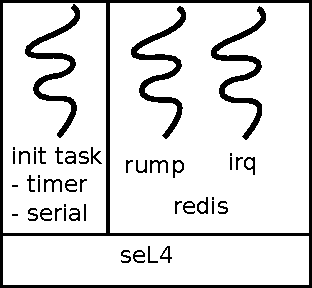
\includegraphics{redis-arch}
    \caption{System architecture of the Redis / \gls{YCSB} benchmark on \selfour, 
        Linux, NetBSD and Rump unikernel.}
    \label{f:redis-arch}
\end{figure}


\cref{t:redis} shows the achieved throughput of Redis+Rump
running  bare-metal, and Redis on the \selfour baseline and as well as the MCS
branch, plus Linux and NetBSD for comparison.

The utilisation figures show that the system is fully loaded, except
in the Linux case, where there is a small amount of idle time. The
cost per operation (utilisation over throughput) is best on Linux, a
result of its highly optimised drivers and network stack. Our
bare-metal and \selfour-based setups use Rump's NetBSD drivers, and
actually achieve slightly better performance than NetBSD. This
indicates that the MCS model comes with low overhead.

\begin{table}[t]\centering
      \rowcolors{3}{}{gray!25}
      \begin{tabularx}{\textwidth}{Xrrrrr}\toprule
          \emph{System}   & \emph{IRQ} & \emph{Throughput} & \emph{Utilisation} & \emph{Cost} & \emph{Latency} \\
                          &            & (k ops/s)         & (\%)               & per op.     & (ms)            \\
        \midrule

      \input{data/ycsb-redis.inc}
      \bottomrule
    \end{tabularx}
    \caption{Throughput (k\,ops/s) achieved by Redis using the YCSB
      workload A with 2 clients.  Latency is the average Read and Update,
      standard deviations in parentheses and omitted where less than the least
      significant digit shown.}
    \label{t:redis}
\end{table}

\subsection{Summary}

All in all, we have demonstrated via micro- and macro- benchmarks that our overheads are
reasonable given the speed of the baseline kernel and the extend of the provided
functionality. 
\clearpage

\section{Temporal Isolation}

We now evaluate the temporal isolation properties achieved by the model described in TODO. We use
two system benchmarks to show that processes attain and do not exceed their
CPU allocation provided by their scheduling context. We then evaluate and demonstrate different
techniques to restore server state after a timeout exception and finally show temporal isolation between
clients in a shared server scenario.

% Show isolation between processes using different scheduling contexts
\subsection{Process isolation} 

We evaluate process isolation, where processes do not share resources, indirectly via network
throughput and network latency in two separate benchmarks. 

\subsubsection{Network throughput}

First, we demonstrate our isolation properties with the Redis setup described in
\Cref{s:evaluation-redis-overhead} with an additional, high-priority active CPU-hog thread
competing for \gls{CPU} time.  All scheduling contexts in the system are configured with a
5\,ms period. We use the budget of the hog to control the amount of time left over
for the server configuration. \autoref{f:redis} shows the throughput
achieved by the YCSB-A workload as a function of the available CPU
bandwidth (i.e \ the complement of the bandwidth granted to the hog
thread). Each data point is the average of three benchmark runs.

\begin{figure}[h]
  \centering
  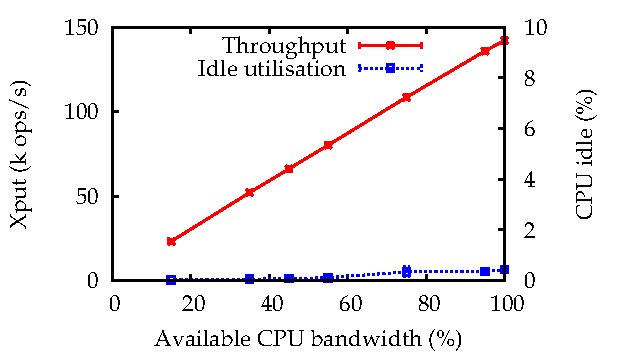
\includegraphics{redis}
  \caption{Throughput of Redis YCSB workload A and idle time vs available bandwidth.}
  \label{f:redis}
\end{figure}

The graph shows that the server is CPU limited (as indicated by very low idle time)
and consequently throughput scales linearly with available CPU
bandwidth.

\subsubsection{Network latency}

Second, we evaluate process isolation via network latency in a system shown in \cref{f:ipbench-arch}. 
The system consists of a single-core of a Linux \gls{VM} which runs at a high priority with a
constrained budget and a \gls{UDP} echo server running at a lower priority,
representing a lower-rate \textsc{high} thread. We
measure the average  and maximum UDP latency reported by the
ipbench~\citep{Wienand_Macpherson_04} latency test.

\begin{figure}[h]
    \centering
    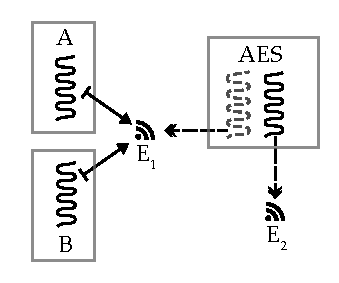
\includegraphics{ipbench-arch}
    \caption{System architecture of ipbench benchmark.}
    \label{f:ipbench-arch}
\end{figure}


Specifically, the Linux VM interacts with timer (PIT) and serial device drivers implemented as
passive servers outside the \gls{VM}; all three components are at a high priority. In the Linux server we
run a program (\code{yes > /dev/null}) which consumes all available
CPU bandwidth.  The UDP echo server, completely isolated from the Linux instance during the
benchmark, but sharing the
serial driver, runs at a low priority with its own HPET timer
driver.

Two client machines run ipbench daemons to send packets to the UDP-echo server on the target machine
(\textsc{x64}). The control machine, one of the load generators, runs ipbench with a \gls{UDP} socket at 10\,Mbps over a 1\,Gb/s Ethernet connection with 100-byte packets. The Linux VM has a 10\,ms period and we vary the
budget between 1\,ms and 9\,ms.
We represent the zero-budget case by an unconstrained Linux that is not running any user code.
Any time not consumed by Linux is available to UDP echo for processing
10,000 packets per second, or 100 packets in the time left over from
each of Linux's 10\,ms period.

\autoref{f:ipbench} shows the average and maximum \gls{UDP} latencies for
ten runs at each budget setting. We can see that the maximum latencies
follow exactly the budget of the Linux server (black line) up to 9\,ms. Only
when Linux has a full budget (10\,ms), and thus able to monopolise the
processor, does the UDP server miss its deadlines, resulting in a
latency blowout.  This result shows that our sporadic server implementation is effective in bounding interference of a high-priority process.

\begin{figure}[h]
  \centering
  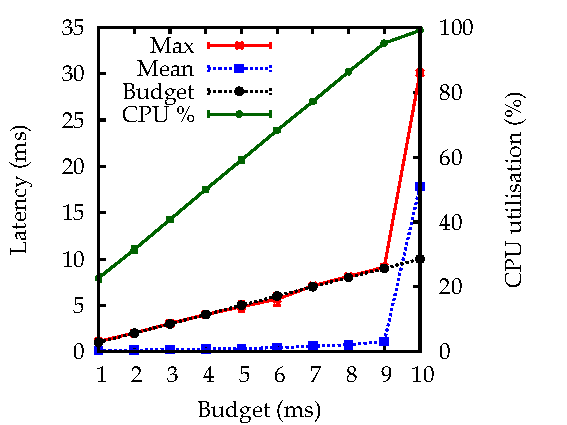
\includegraphics{ipbench}
  \caption{Average and maximum latency of UDP packets with a CPU hog running a high priority with a 10\,ms budget.}
  \label{f:ipbench}
\end{figure}

% Show isolation in a shared server
\subsection{Server isolation} 
\label{s:server-isolation}

To demonstrate temporal isolation in a shared server, we use a case study of an encryption service
using \gls{AES} to encrypt client data. We measure both the overhead of different recovery techniques, and the
throughput achieved when two clients constantly run out of budget in the server.

\Cref{f:aes-arch} shows the architecture of the case study. Both clients $A$ and $B$ are single
 threaded and exist in separate address spaces to the server. The server has two threads, a passive
 thread for serving request on the clients scheduling context and an active thread which handles
 timeout exceptions for the server. The server and timeout exception handler share the same virtual
 memory and capability spaces.

\begin{figure}
\centering
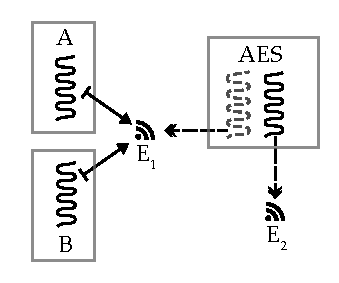
\includegraphics{aes-arch}
\caption{Architecture of the \gls{AES} case study. Client $A$ and $B$ make \gls{IPC} requests over
endpoint $E_{1}$ of passive $AES$ which has an active timeout fault handling thread waiting for
fault \gls{IPC} messages on endpoint $E_{2}$.}
\label{f:aes-arch}
\end{figure}

The server itself runs the AES-256 algorithm with a block size of 16~bytes. The server alternates between two
buffers using an atomic swap, of which one always contains consistent state, the other is
dirty during processing. When a timeout fault occurs only the dirty buffer is lost due to
inconsistency. 

Both clients request 4\,MiB of data to be encrypted, and have a budget insufficient to
complete the request. When the server is running on the clients scheduling context and the budget
expires, a timeout exception, which is a fault IPC message from the kernel, is delivered to the timeout
handler. 

\subsection{Timeout handling techniques}

If client scheduling context is depleted while the server is servicing the request, a timeout fault is raised and
sent to the timeout handler.
The appropriate protocol for handling such faults depends ultimately on the requirements of the system.
Consequently, we implement and evaluate four different timeout fault handling techniques: rollback, error,
emergency and extend. 

While each technique is evaluated separately, combinations of such techniques could be used for
different clients depending on their requirements. For example, trusted clients may get special
treatment. Note that in all cases of blocking IPC, clients must trust the server as discussed in
TODO. Additionally, although out experiment places the timeout fault handler in the server's address
space, this is not necessary: for approaches that require access to scheduling contexts and
scheduling control capabilities, the timeout handler may be placed in a scheduling servers address
space, separate from the server itself.

\subsubsection{Rollback}

Rollback restores the server to the last known consistent state recorded. In the case of non-thread
safe servers, this may require rolling back an entire request. However, algorithms like \gls{AES}
which can easily be batched can make progress. The process for rollback involves is as follows:

\begin{enumerate}\label{e:rollback}
    \item Fault is received by timeout handler.
    \item Handler replies to the client by sending a message to the client reply
        object, with an indication of how much progress has been made. In the case of \gls{AES} this
        is how much data is left to encrypt. By invoking the reply object, the client's
        scheduling context is returned from the server to the client.
    \item Server is restored to a known state by the timeout handler (restoring registers, stack
        frames and any global state. 
    \item Handler binds a scheduling context to the server for it to execute on.
    \item Handler blocks waiting for a message from the server.
    \item Now the server runs from its checkpoint. In the case study, the server is checkpoint just
        before it initiates the passive initialisation protocol (TODO ref to passive init figure), so this system call is
        repeated. The server signals the timeout handler and blocks on $E_{1}$, ready for client
        requests.
    \item Handler wakes and converts the server back to passive.
    \item Handler blocks on $E_{2}$, ready for further timeout faults.
\end{enumerate}

The rollback technique requires the server and timeout handler to both have access to the reply
object that the server is using, and the servers \gls{TCB}, meaning the timeout handler must be
trusted by the server. In our example the server and timeout handler run at the same priority, in
all cases both must run at higher priorities than the clients. 

Once the budget of the faulting client is replenished it can then continue the request based on the
content of the reply message sent by the timeout handler. Clients are guaranteed progress as long as
their budget is sufficient to complete a single batch of progress.

If rollback is not suitable, the server can be similarly reset to the initial state and an error
returned to the client. However this does not guarantee progress for clients with insufficient
budgets.

\subsubsection{Kill}

In cases of non-preemptible servers, potentially due to a lack of thread safety, one option is to
kill client threads. Such a scenario would stop untrusted misbehaving clients from constantly
monopolising server time.  We implement an example were the timeout handler has access to client \gls{TCB}
capabilities and simply calls suspend, however the server could also switch to a new reply object
and leave the client blocked forever, without access to any of the clients capabilities. 

The process for suspending the client is the same as that for \Cref{e:rollback} but for two aspects;
the server state does not need to be altered by the timeout handler as the server always 
restores to the same place, and instead of replying to the client it is suspended.

\subsubsection{Emergency}

Another technique gives the server a one-off emergency budget to finish the client request, after
which the exception handler resets the server to being passive. This could be used in low
criticality \gls{SRT}
scenarios where isolation is desired but transient overruns are expected.
An example emergency protocol follows:

\begin{enumerate}\label{e:emergency}
    \item Fault is received by timeout handler.
    \item Unbind client scheduling context from server. \TODO{clarify who does what}
    \item Bind server with emergency budget.
    \item Reply to the timeout fault, which restarts the server.
    \item Enqueue the timeout handler itself, with an empty sized request, in the servers
          endpoint queue, by invoking $E_{1}$
    \item Server finishes request with extra budget and replies to the client.
    \item Timeout handler is highest priority, so it overtakes other clients and wakes up after the 
          server processes its empty request. The handler then converts the server back to passive.
    \item Handler blocks on $E_{2}$, ready for further timeout faults.
\end{enumerate}

This case requires the timeout handler to have access to client scheduling contexts in order to
unbind them from the server. 

\subsubsection{Extend}

The final technique is to simply increase the clients budget on each timeout, which requires the
timeout fault handler to have access to the clients scheduling contexts.
This could be deployed in \gls{SRT} systems or for specific threads with unknown budgets up to a limit. 

\begin{enumerate}\label{e:extend}
    \item Fault is received by timeout handler.
    \item Extend client budget by configuring scheduling context.
    \item Reply to fault message, which resumes the server.
\end{enumerate}

\subsection{Results}

We measure the pure handling overhead in each case, from when the timeout handler wakes up to when it blocks again. 
 Given the small amount of rollback state, this measures the baseline
    overhead. For schedulability analysis, the actual cost of the rollback would
have to be added, in addition to the duration of the timeout fault IPC. 
 
We run each benchmark with hot caches (primed by some warm-up
iterations)  as well as cold (flushed) caches and measure the 
latency of timeout handling, from the time the handler wakes up
until it replies to the server.

\autoref{t:rollback} shows the results. The maximum
cold-cache cost, which is relevant for schedulability analysis,
differs by a factor of 3--4 between the different recovery scenarios,
indicating that all are about equally feasible.
Approaches that restart the server and send \glspl{IPC} messages on its behalf (rollback, reply) are the most expensive
as they must restore the server state from a
checkpoint and follow the passive server initialisation protocol
(recall \autoref{s:passive}). 

\begin{table}[t]\centering
\begin{tabular}{cllrrrr}\toprule
\emph{Platform} & \emph{Operation} & \emph{Cache} & \emph{Min} &
                          \emph{Max} & \emph{Mean} &
                          \multicolumn{1}{c}{\boldmath \(\sigma\)} \\\midrule
                          \multirow{8}{*}{\textsc{Sabre}} 
                          \input{data/generated/sabre-aes.inc} 
                          \midrule
                          \multirow{8}{*}{\textsc{x64}}
                          \input{data/generated/haswell-aes.inc}
                          \bottomrule
\end{tabular}
\caption{Cost of timeout handler operations in \(\mu\)s, as measured
  by timeout exception handler. \(\sigma\) is the standard deviation.}
\label{t:rollback}
\end{table}

\subsection{Rollback isolation}

We next demonstrate temporal isolation in the server by using the rollback
technique and measuring the time taken to encrypt 10 requests of 4\,MiB of
data. \autoref{f:aes} shows the result with both clients having the same
period, which we vary between 10\,ms and 1000\,ms.
In each graph we vary the clients' budgets between 0 and the
period. The extreme ends are special, as one of the clients has a full
budget and keeps invoking the server without ever getting rolled back,
thus monopolising the processor. In all other cases, each client
processes at most 4\,MiB of data per period, and either succeeds (if
the budget is sufficient) or is rolled back after processing less than 4\,MiB.

\begin{figure*}[t]
  \centering
  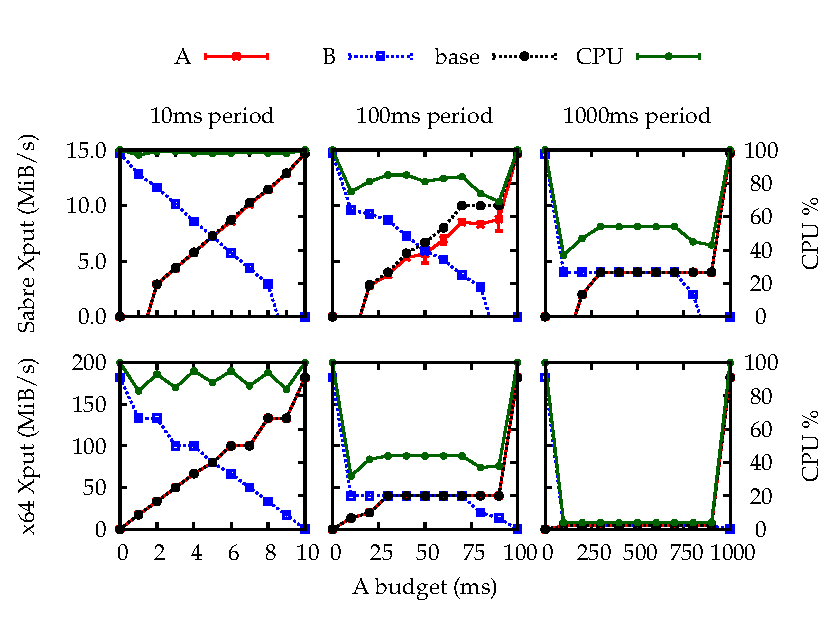
\includegraphics{aes-shared}
  \caption{Throughput for clients A and B of a passive AES server processing 10 requests of 4\,MiB of data with
      limited budgets on the \textsc{x64} (top row) and \textsc{sabre} (bottom row) platforms. The two clients' budgets
      add up to the period, which is varied between graphs (10, 100, 1000\,ms). Clients sleep when
      they process each 4\,MiB, until the next period, except when their budgets are full. Each data point is the average of 10 runs, error bars show the standard deviation.}
  \label{f:aes}
\end{figure*}


The results show that in the CPU-limited cases (left graphs)
we have the expected near perfect proportionality between throughput and
budget (with slight wiggles due to the rollbacks), showing isolation between clients. In the cases where there is headspace (centre of the right
graphs), both clients achieve their desired throughput.

\subsection{Summary}

%TODO rewrite to align with goals at start of chapter
Through two system benchmarks and one shared-server benchmark, we have shown that our approach
guarantees processor isolation and that threads cannot exceed their budget allocation via their
scheduling context. Additionally we have shown that isolation can be achieved in a shared server via
a timeout fault handler and demonstrated several alternatives for handling such faults,
demonstrating the feasibility of the model. 

\section{Asymmetric Protection}

We evaluate our kernel mechanism for changing criticality
with two benchmarks: A
microbenchmark measuring the cost of a mode switch, and another showing deadline misses of threads sets over several mode changes.

\begin{figure}[t]
  \centering
  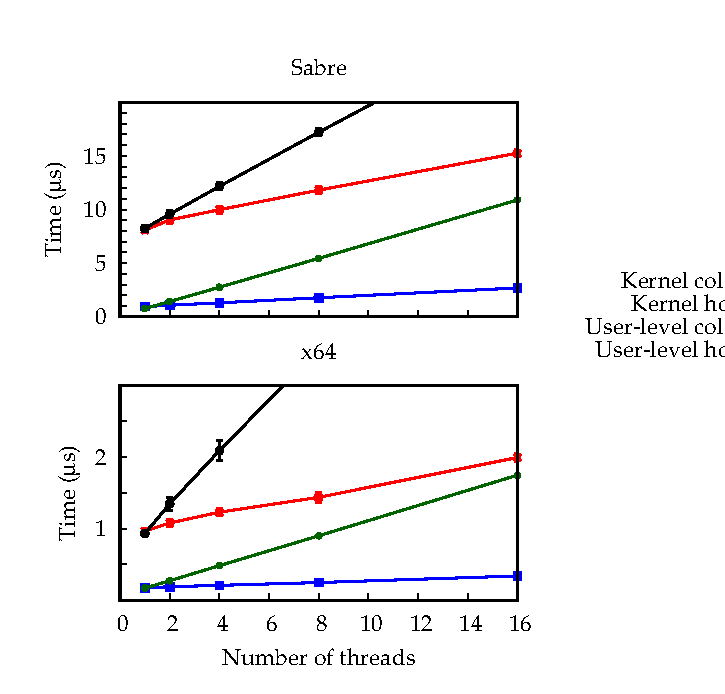
\includegraphics[width=\linewidth]{mode-switch-all}
  \caption{Cost of switching the priority of $n$ threads, as well as changing from \crit{low} to
  \crit{high} criticality level while increasing the number of \crit{high} and \crit{low} threads,
  on \textsc{sabre} and \textsc{x64}. Each data point is the average of 100 runs, with very small standard
  deviations.}
  \label{f:mode-switch}
\end{figure}

To evaluate the cost of changing the system criticality level, we
configure the kernel with 128 priorities and 2 criticality levels
(0--1). We then  run 3 experiments as follows:
\begin{description}
    \item[\textsc{UL}:] measures the time to change the priority of $n$ threads from user-level;
    \item[\textsc{HI}:] measures the time for raising the system criticality level from 0 to 1 with one \crit{low} thread and $n$
    \crit{high} threads, i.e.\ the priority of $n$ threads must be boosted;
\item[\textsc{LO}:] measures the time for raising the system criticality level from 0 to 1 with one \crit{high} thread and
    $n$ \crit{low} threads, i.e.\ only one thread must be boosted.
\end{description}

\Cref{f:mode-switch} shows the results, where each data point is the result of 100 measurements.
We show results with a primed cache (hot) and flushed cache (cold).
As the graph shows, switching is linear in the number of \crit{high} threads being boosted. Varying the number
of \crit{low} threads has no impact on the execution time of a mode switch.
This is important, as the schedulability analysis for critical threads
must not depend on less-critical threads, and should not make
assumptions how many threads less-critical software creates.

In absolute terms, the results show that a mode switch is fairly fast,
remaining under 2\,$\mu$s on \textsc{x64} and about 12\,\(\mu\)s on \textsc{sabre} for switching 8 threads
with a cold cache. Most systems will not have more than a few high
criticality threads, and deadlines for critical control loops in
cyber-physical systems tend to be in the tens of milliseconds, meaning
that budgeting a few microseconds for an emergency mode switch is eminently
feasible.

Additionally, the results show that changing the priority at user-level, rather than using the
criticality boost, is also linear in the number of threads to be boosted, but  is significantly slower than using the kernel mechanism (i.e.\ mode switch).
The higher cost from user-level operation results from  multiple switches between kernel and user mode, and the repeated thread-capability look-ups.

% TODO mode switch benchmark
For our second mode-switch benchmark, we ported 3 processor intensive benchmarks from the
MiBench~\citep{Guthaus_REAMB_01} to act as workloads. Each benchmark runs in its own Rump process
with an in-memory file system, and shares a timer and serial server.

We altered the benchmarks to run periodically in multiple stages. To obtain
execution times long enough, some of the benchmarks iterate a fixed number of times per
stage. Each benchmark process executes its workload and then waits for the next period to start.
Deadlines are implicit: if a periodic job finishes before the start of the next period it is
considered successful, otherwise the deadline is missed.

\Cref{t:modeswitch} lists the benchmarks with periods and criticalities.
\textit{susan}, the most critical, has three stages: edge detection, smoothing, and corners. The
next critical task, \textit{jpeg}, has two stages: encode, and decode. The least
critical task, \textit{mad} has only one stage. We run the benchmark
for 20\,s for each of the stages (repeating the last phase where
threads have no new phase), and
increment the system criticality level at stage transition. The parameters are arranged such that
rate-monotonic priorities are inverse to the criticalities.

Results are shown in \autoref{t:modeswitch}. For stage one, the entire workload is schedulable and
there are no deadline misses. For stage two, the workload is not
schedulable, and the criticality switch boosts the priorities of
\textit{susan} and \textit{jpeg}, such that they meet
their deadlines, but
\textit{mad} does not. In the final stage, only the most critical task
meets all deadlines.
This shows that our mechanisms operate as intended.

\begin{table}[h]
    \centering
    \begin{tabular}{lcccccclcl}\toprule
        \emph{Application} & \emph{T} & \emph{L} & \emph{\(L_S\)} & \emph{C} & \emph{U} & \emph{j} &
        & \emph{m}  & \\\midrule
        \input{data/generated/mode_switch.inc}
        \bottomrule
    \end{tabular}
    \caption{Results of mode switch benchmark for each
        stage, where the  criticality \(L_S\) is raised each stage. \(T\) =
        period, \textit{C} = worst observed execution time (ms),
      \textit{U} = allowed utilisation (budget/period),
      \textit{m} = deadline misses, \textit{j} = jobs completed. We recorded 52 (0.1), 86 (15.2)
      and 100 (0.0)\% CPU
utilisation for each stage respectively. Standard deviations are shown in parenthesis.}
    \label{t:modeswitch}
\end{table}


\section{Practicality}

\TODO{intro}

\subsection{User-level scheduling}\label{s:edf-impl}

Fundamental to the microkernel philosophy is keeping policy out of the
kernel as much as possible, and instead providing general mechanisms
that allow the implementation of arbitrary policies
\citep{Heiser_Elphinstone_16}.  As on the face of it, our
fixed-priority-based model seems to violate this principle,  we
demonstrate that the model is general enough to support the efficient
implementation of alternate policies at user level. Specifically, we
show that we can efficiently implement \gls{EDF}, the popular and  optimal dynamic-priority policy (see \autoref{s:theory}).

We implement the EDF scheduler as an active server with active
clients which run at an \selfour priority below the scheduler.
The scheduler waits on an endpoint on which it receives messages from
its clients or the timer.

Each client has a period which represents its relative deadline and a full reservation (i.e.\ equal to the period). Clients
either explicitly notify the scheduler of completion by an IPC
message, or else create a timeout exception on preemption, which is also received by the
scheduler. Either is an indication that the next thread should be scheduled.

We use the \emph{randfixedsum}~\citep{Emberson_SD_10} algorithm to
generate deadlines between 10 and 1000\,ms for a certain number of threads.
A set of threads runs until 100
scheduling decisions have been recorded. We repeat this 10 times,
resulting in 1,000 scheduler runs for each data point.

We measure the scheduler latency by recording the timestamp when each client thread, and an idle
thread, detects a
context switch and processing the difference in timestamp pairs offline. We run two schedulers:
\emph{pre}-empt where threads never yield and must incur a timeout exception, and \emph{coop}, where
threads use IPC to yield to the scheduler. The latter invokes the user level timer
driver more often as the release queue is nearly always full, which involves more kernel invocations
to acknowledge the IRQ, in addition to reprogramming the timer.

We compare our latencies to those of
LITMUS$^{RT}$~\citep{Calandrino_LBDA_06}, a widely-used real-time scheduling
framework embedded in Linux, where we use Feather-Trace~\citep{Brandenburg_Anderson_07} to gather data.
We use the C-EDF scheduler, which is a partitioned (per-core), clustered (per-node) EDF scheduler, on a single
core. We use the same parameters and thread sets, running each set for 10\,s. 
The measured overhead considers the in-kernel scheduler, context-switch and user-level code to return to
the user.

\autoref{f:edf} shows that our user-level EDF scheduler implementation is
competitive with t EDF from LITMUS$^{RT}$, and
that the cost of implementing scheduling policy at user level is of
the same order as the in-kernel default scheduler. In other words,
implementing different policies on top of the base scheduler is quite feasible.

\begin{figure}[t]
    \centering
    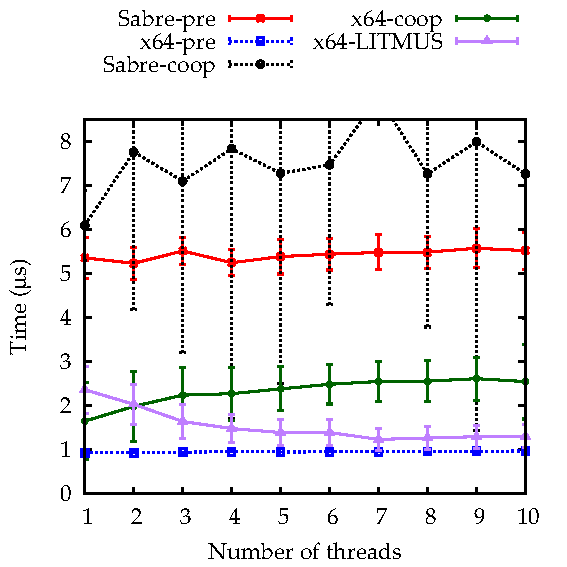
\includegraphics{edf}
    \caption{Execution time of \selfour user-mode EDF scheduler compared to
             kernel scheduler in \textsc{x64} LITMUS$^{RT}$.}
    \label{f:edf}
\end{figure}

\subsection{Multicore}

We run two multicore benchmarks, the first evaluating multicore throughput of the MCS kernel vs. the
baseline kernel, the second based on our shared server \gls{AES} case study to demonstrate the
multicore model. 

\subsubsection{Throughput}

We run an multicore throughput benchmark to show that our MCS model
avoids introducing scalability problems on multiple cores compared to the baseline kernel.
We modify the
existing multicore IPC throughput benchmark for \selfour to run on the MCS kernel. 
At time of writing, only \textsc{x64} and \textsc{sabre} have \selfour multiprocessor support, 
consequently these are the platforms used for the benchmark.

The existing multicore benchmark measures IPC throughput of a client and server, both 
pinned to the same processor, sending fastpath, 0 length IPC messages of via \call
and \replyrecv. One pair of client and server is set up per core. Both threads are
the same priority and the messages are 0 length. Each thread spins for a random amount
with an upper bound \textit{N} between each subsequent IPC. As \textit{N} increases so does
IPC throughput, as less calls are made.

We modify the benchmark such that each server thread is passive on the MCS kernel.
Results are displayed in \Cref{f:evaluation-smp} and show a minor impact on IPC throughput
for high values of \textit{N}. Scalability is not impacted on \textsc{sabre}, but is on \textsc{x64},
with the curve flattening slightly more aggressively on the MCS kernel
due to the fastpath overhead. This is expected as the MCS model only introduces extra 
per-core state, with no extra shared state between cores.

\begin{figure}[ht] 
    \centering
    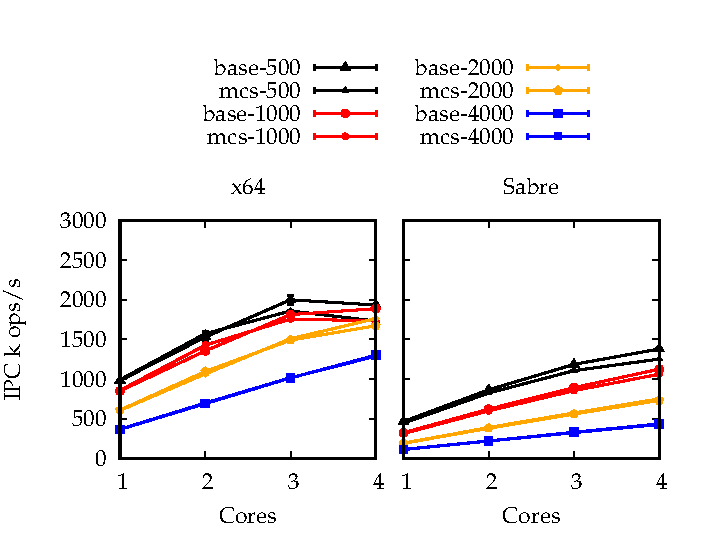
\includegraphics{smp}
    \caption{Results of the multicore IPC throughput benchmark, baseline \selfour vs MCS. 
        Each series is named \textit{name-N}, where \textit{name} is \textit{base} and \textit{mcs} for 
        the baseline and MCS kernel respectively, and \textit{N} is the upper
        bound on the number of cycles between each IPC for that series.}
    \label{f:evaluation-smp}
\end{figure}

\subsubsection{Shared server}

We adapt our \gls{AES} case study (\cref{s:server-isolation}) to demonstrate how our MCS model 
applies to multiprocessors. The AES server is configured without a timeout fault handler, and
we run two variants. 

\begin{description}
    \item[Single:] the AES server has a single passive thread, which waits on a single endpoint
        and migrates to the core of the active client over IPC, effectively serialising access to the server.
        Consequently, \cref{f:evaluation-smp-aes} shows there is no gain in throughput when further cores are
        added. 
    \item[Multiple:] the AES server has one passive thread per core, and an endpoint is set up for
        each core, demonstrating a parallel server. Due to minimal bottlenecks in the stateless 
        AES server, this results in near perfect scalability.
\end{description}

\begin{figure}[ht] 
    \centering
    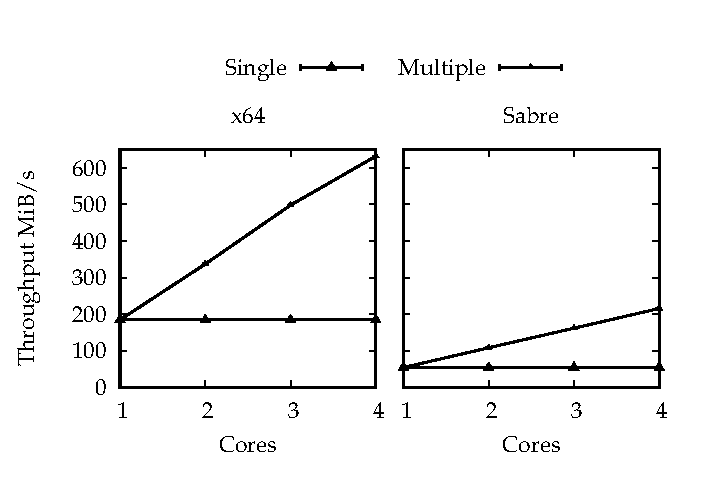
\includegraphics{smp_aes}
    \caption{Results of the AES shared server multicore case study. \emph{Single} shows results for a 
        passive server thread migrating between cores to service clients, while \emph{Multiple} has one
        passive server thread per core. For both series, the number of clients is equal to the number of
        cores and each client requests 1MiB of data encrypted. }
    \label{f:evaluation-smp-aes}
\end{figure}


\section{Summary}

% TODO summarise eval
Our evaluation demonstrates our model has minimal overheads, achieves isolation,  provides a notion
of criticality orthogonal to priority, and allows for efficient user-level scheduling.
In total, we add 2,245 lines of SLOC~\citep{Wheeler_01} to the preprocessed kernel code for the \textsc{sabre}
(the verified platform), representing a 16\% increase.

